\documentclass[a4paper,12pt]{article}
\usepackage{graphicx}
\usepackage{fancyhdr}
\usepackage{geometry}
\usepackage{hyperref}
\usepackage{float} 

% Page setup
\geometry{top=1in, bottom=1in, left=1in, right=1in}
\pagestyle{fancy}
\fancyhead[L]{AgriVision Design Document}
\fancyhead[C]{}
\fancyhead[R]{Version 1.0}

% Configure hyperref to remove borders
\hypersetup{
    hidelinks,       % Removes link colors and borders
    colorlinks=false % Ensures links are clickable but not visible
}

\documentclass[12pt]{article}
\usepackage{graphicx}
\usepackage{longtable}
\usepackage{geometry}
\usepackage{titlesec}
\usepackage{enumitem}
\usepackage{fancyhdr}
\usepackage{tocloft} % For customizing the table of contents
\usepackage{makeidx} % For creating an index

% Set margins
\geometry{margin=1in}

% Title formatting
\titleformat{\section}{\large\bfseries}{\thesection}{1em}{}
\titleformat{\subsection}{\bfseries}{\thesubsection}{1em}{}

% Header and footer setup
\pagestyle{fancy}
\fancyhf{}
\fancyhead[L]{Resource Sharing Web Application}
\fancyhead[R]{\thepage}

% Title and author information
\title{\textbf{RAJIV GANDHI UNIVERSITY OF KNOWLEDGE TECHNOLOGIES\\BASAR,NIRMAL\\
		TELANGANA-504107}\\}
\date{}

% Customizing the Table of Contents and List of Figures
\renewcommand{\cftsecfont}{\bfseries} % Bold section titles
\renewcommand{\cftsubsecfont}{\itshape} % Italicize subsection titles
\renewcommand{\cftsecleader}{\hfill} % Fill space between section title and page number
\renewcommand{\cftfigfont}{\bfseries} % Bold figure titles
\renewcommand{\cftfigleader}{\hfill} % Fill space between figure title and page number

% Create index


\begin{document}
\maketitle
\begin{center}
	\textbf{DEPARTMENT OF COMPUTER SCIENCE ENGINEERING}
\end{center}
\begin{figure}[h]
	\centering
	
\includegraphics[width= 8 cm]{logo1.jpeg}
\end{figure}

% SRS Title
\begin{center}
	\textbf{\huge  Software Design Document}\\[.5cm] \textbf{for} \\[0.5cm]	\textbf{\huge Agri vision}\\[1cm]
\end{center}


\begin{center}
	% Team Members and IDs
	\textbf{ Prepared by:}\\[0.5cm]
	\textbf{Depavath Naresh [B200391 ]}\\[0.5cm]
	\textbf{Mudavath kalyan  [B201174]}\\[0.5cm]
	\textbf{Mudapally Aravind. [B200778]}\\[0.5cm]
\end{center}
\newpage

\begin{document}

\maketitle
\tableofcontents
\newpage

\section{Introduction}

\subsection{Project Overview}
AgriVision is an innovative web application designed to revolutionize the agriculture industry by directly connecting farmers, sellers, and consumers on a single platform. It eliminates the need for intermediaries, ensuring fair pricing and transparent transactions while fostering better communication among stakeholders. The platform offers tailored features for each user role to streamline agricultural operations and enhance productivity.

Farmers can list and manage grains for sale, rent agricultural machinery, and purchase seeds or pesticides directly from sellers. They also have access to real-time weather data through an interactive map, helping them make informed decisions. Sellers can manage their profiles, add or remove products, and provide necessary agricultural supplies to farmers. Consumers can browse available products, purchase directly from farmers, and manage their shopping cart, offering them a seamless buying experience.

The application integrates a powerful AI chatbot to assist users with queries, making the platform user-friendly and accessible. The backend is built with Node.js and Express, while the frontend is developed using React. MongoDB serves as the database, with carefully structured collections to manage users, products, orders, and rentals efficiently.

To enhance the user experience, AgriVision features an intuitive design with dedicated pages for product browsing, cart management, user profiles, and order history. The interactive map for weather insights is implemented using Leaflet.js, and the entire system is deployed using Netlify and Heroku for scalability and reliability.

By connecting farmers, sellers, and consumers directly, AgriVision aims to empower stakeholders, promote transparency, and create a fair agricultural ecosystem. It is a comprehensive solution that leverages modern technology to address challenges in agriculture, making it a vital tool for the agricultural community.

\subsection{Purpose and Scope}
The purpose of the Agri Vision project is to create a unified platform that bridges the gap between farmers, sellers, and consumers in the agriculture industry. By providing features such as interactive weather maps, product management tools, and secure communication channels, the platform aims to streamline agricultural trade and resource management. The project eliminates the need for intermediaries, enabling farmers to sell their products at fair prices and access essential resources like seeds, pesticides, and machinery directly from sellers. Additionally, consumers can purchase high-quality agricultural products with transparency and ease. This fosters a sustainable and efficient agricultural ecosystem.
\begin{itemize}
    \item \textbf{Vulnerability Detection}:The Agri Vision platform is a web-based solution designed to cater to the needs of farmers, sellers, and consumers.
    \item \textbf{Farmers}:Ability to add, delete, and manage agricultural products, view weather updates, and rent machinery or purchase seeds and pesticides..
    \item \textbf{Sellers}:Manage product inventories, edit profiles, and list products for sale to farmers and consumers. 
    \item \textbf{Consumers}: Purchase materials directly from farmers, manage cart items, and leave ratings for products.
    \item \textbf{Integration with External Services}:Additional features include a chatbot for user support, an interactive map for weather insights, and a secure, user-friendly interface. The platform will leverage a modular architecture (MERN stack) to ensure scalability, maintainability, and efficient performance. The scope also extends to improving trust, transparency, and communication among all stakeholders while offering a reliable and efficient system for managing agricultural operations and transactions. .
\end{itemize}

\subsection{Audience}
This document is intended for a diverse group of stakeholders, each with specific interests in the system's design. The following audiences are targeted:
\begin{itemize}
    \item \textbf{Developers}: This document provides a detailed guide on the system's architecture, modules, and interactions, enabling developers to build, extend, and maintain the Agri Vision platform efficiently.
    \item \textbf{System Architects}: System architects can review the proposed design for scalability, security, and performance, ensuring it aligns with the system's goals. The document also provides insights into integration points and infrastructure requirements.
    \item \textbf{Project Managers}: Project managers can utilize this document to oversee project progress, allocate resources effectively, and ensure that the design meets functional and non-functional requirements within the given timeline.
    \item \textbf{Testers}: Testers can use the workflows and design specifications provided in this document to create test cases, ensuring that all system functionalities, including interactive maps, product management, and user roles, are thoroughly validated.
    \item \textbf{Agricultural Stakeholders}: This group includes farmers, sellers, and consumers who will benefit from a high-level understanding of the system’s capabilities, such as product management, direct transactions, and weather-based insights.
    \item \textbf{End Users}: A high-level overview in this document will help end users comprehend features like chatbot interactions, weather updates, and seamless buying/selling of agricultural products.
\end{itemize}


\subsection{Key Features and Benefits}
Agri Vision is designed with several features to connect farmers, sellers, and consumers, ensuring efficient resource management and direct transactions:
\begin{itemize}
    \item \textbf{Interactive Weather Map}: Users can click on a map to access real-time weather updates for their specific location, aiding in better agricultural planning and decision-making.
    \item \textbf{Chatbot Assistance}: The integrated chatbot provides instant support for users, answering queries about the platform’s features, processes, and navigation.
    \item \textbf{Role-Based Profiles}: Separate profiles for farmers, sellers, and consumers allow tailored functionalities such as adding/deleting products, renting machines, and managing orders.
    \item \textbf{Streamlined Transactions}: Farmers can sell grains directly to consumers, purchase seeds/pesticides, or rent machinery without intermediaries, ensuring fair pricing and efficiency.
    \item \textbf{Scalable Platform}: Agri Vision is designed to accommodate multiple users and transactions, making it suitable for diverse agricultural communities.
    \item \textbf{Secure and User-Friendly Design}: The platform ensures data privacy for all users while offering a simple interface to encourage widespread adoption and ease of use.
\end{itemize}


\subsection{System Requirements}
The system operates within the following requirements:
\begin{itemize}
    \item \textbf{Software Requirements}:
    \begin{itemize}
        \item Server: Linux or Windows-based environment (Ubuntu, CentOS, or Windows Server)
        \item Backend: Node.js with Express.js for API handling
        \item Frontend: React.js for building dynamic and interactive user interfaces
        \item Database: MongoDB for storing user profiles, product information, and transaction data
        \item Mapping and Weather APIs: OpenStreetMap and a weather API (such as OpenWeather) for real-time location and weather updates
    \end{itemize}
    \item \textbf{Hardware Requirements}:
    \begin{itemize}
        \item A server with at least 4 GB of RAM and a multi-core processor for handling concurrent user requests
        \item Internet connectivity to fetch weather data, interact with APIs, and support real-time chat features
    \end{itemize}
\end{itemize}

\subsection{System Limitations}
Although Agri Vision provides a comprehensive platform for the agricultural sector, it has the following limitations:
\begin{itemize}
    \item \textbf{API Dependency}: The system relies on third-party APIs for weather and mapping data. Any changes or outages in these services can impact the functionality.
    \item \textbf{Resource Constraints}: Real-time updates and transactions may experience delays under heavy user loads or insufficient server resources.
    \item \textbf{Geographical Limitations}: Weather data and mapping services may not provide detailed or accurate information for remote or underdeveloped regions.
    \item \textbf{User Onboarding}: Initial adoption may be limited by the digital literacy of the target audience, particularly farmers unfamiliar with technology.
\end{itemize}


\section{System Architecture}

\subsection{High-Level Overview}
Agri Vision consists of several key components that work together to provide a unified platform for farmers, sellers, and consumers:
\begin{itemize}
    \item \textbf{Frontend}: The user interface (UI) for interactions, built using React.js. It includes components for maps, weather information, user profiles, and product management.
    \item \textbf{Backend}: The server-side logic is implemented with Node.js and Express.js, handling API requests, authentication, and business logic.
    \item \textbf{Database}: MongoDB is used to store user profiles, product details, orders, and transaction history in a scalable and efficient manner.
    \item \textbf{Mapping and Weather Services}: OpenStreetMap integrated with Leaflet provides an interactive map interface, while a weather API fetches real-time weather data.
    \item \textbf{ChatBot Service}: AI-powered chatbot for assisting users in navigating the platform and addressing their queries.
\end{itemize}

\subsection{Technology Stack}
\begin{itemize}
    \item \textbf{Frontend}: React.js for creating a dynamic and interactive user experience.
    \item \textbf{Backend}: Node.js and Express.js for server-side processing and API management.
    \item \textbf{Database}: MongoDB for managing data related to users, products, orders, and weather reports.
    \item \textbf{Mapping Service}: OpenStreetMap and Leaflet.js for rendering maps and enabling location-based features.
    \item \textbf{Weather Service}: Integration with a weather API such as OpenWeather for real-time weather updates.
    \item \textbf{ChatBot}: AI chatbot built with frameworks like Dialogflow or Rasa for user assistance.
\end{itemize}


\newpage

\section{Database Design}

\subsection{Entity-Relationship Diagram (ERD)}
The \textbf{Entity-Relationship Diagram (ERD)} defines the structure of the database, the relationships between various entities, and their attributes. Below is the diagram that explains the database structure for Agri Vision:

\begin{figure}[htbp] % Relaxed float placement with 'htbp'
    \centering
    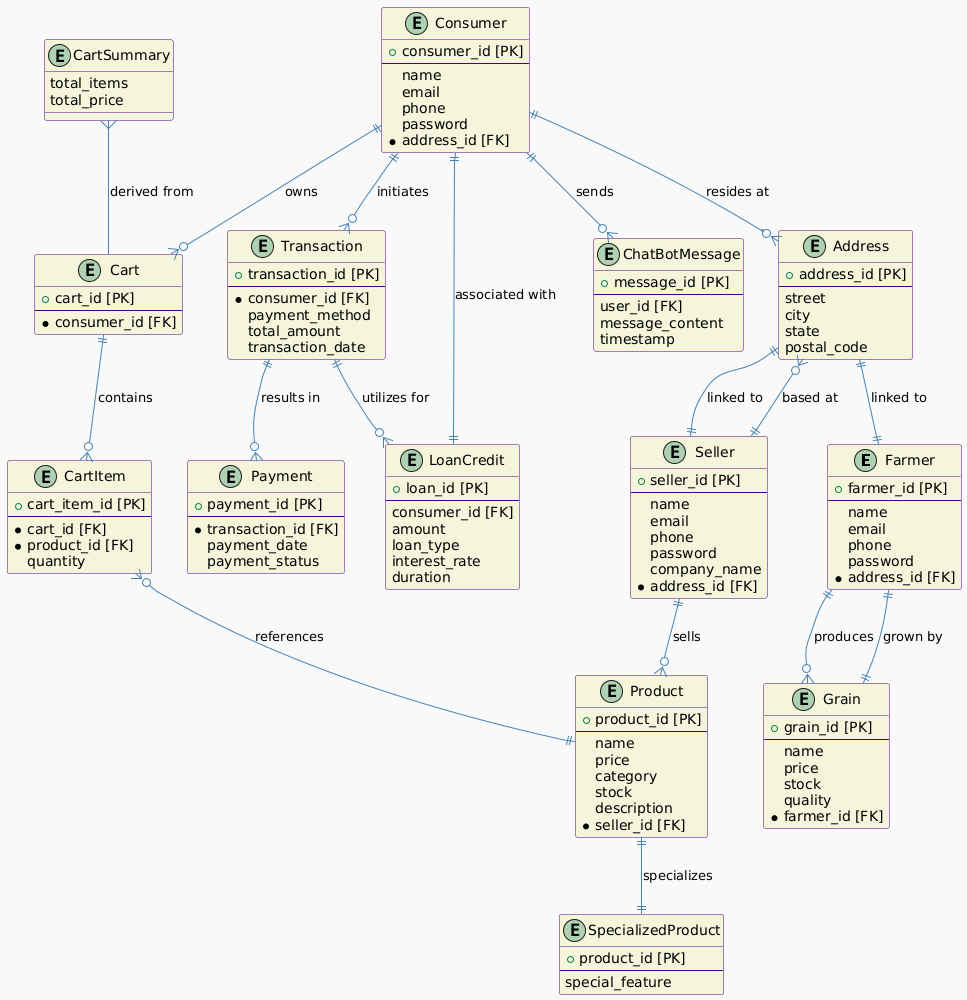
\includegraphics[width=1\textwidth]{ER.png}
    \caption{Main Entity-Relationship Diagram (ERD)}
\end{figure}

\textbf{Explanation}:
\begin{itemize}
    \item \textbf{User Entity}: Represents all system users, including farmers, sellers, and consumers, with attributes like \texttt{userID}, \texttt{name}, \texttt{email}, \texttt{password}, \texttt{role}, and \texttt{address}.
    \item \textbf{Product Entity}: Represents products listed for sale by farmers or sellers with attributes like \texttt{productID}, \texttt{name}, \texttt{description}, \texttt{category}, \texttt{price}, and \texttt{quantity}.
    \item \textbf{Order Entity}: Represents orders placed by consumers, including attributes like \texttt{orderID}, \texttt{productID}, \texttt{consumerID}, \texttt{quantity}, and \texttt{orderStatus}.
    \item \textbf{Weather Data Entity}: Represents weather information for various locations, including attributes like \texttt{locationID}, \texttt{latitude}, \texttt{longitude}, \texttt{temperature}, and \texttt{forecast}.
    \item \textbf{Rental Machine Entity}: Represents machinery available for rent, with attributes like \texttt{machineID}, \texttt{name}, \texttt{description}, \texttt{rentalPrice}, and \texttt{ownerID}.
    \item \textbf{ChatBot Log Entity}: Represents user interactions with the chatbot, including attributes like \texttt{logID}, \texttt{userID}, \texttt{timestamp}, and \texttt{queryResponse}.
\end{itemize}

\textbf{Relationships}:
\begin{itemize}
    \item A \texttt{User} can list multiple \texttt{Products} or \texttt{Rental Machines}.
    \item A \texttt{Consumer} can place multiple \texttt{Orders}.
    \item Weather data is linked to geographic locations, enabling weather reporting for specific regions on the map.
    \item A \texttt{ChatBot Log} is associated with a specific \texttt{User}.
\end{itemize}



\subsection{Sub-Diagrams}

\subsubsection{Farmer Entity Sub-Diagram}

This diagram further breaks down the \textbf{User Entity} to show how the farmer’s profile and preferences are managed.

\begin{figure}[htbp] % Relaxed float placement with 'htbp'
    \centering
    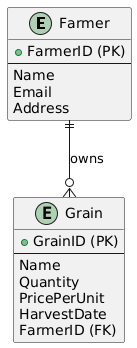
\includegraphics[height=0.5\textwidth]{FARMER_ER.png}
    \caption{Farmer Entity-Relationship Diagram (ERD)}
\end{figure}

\textbf{Explanation}:
\begin{itemize}
    \item The \textbf{Farmer Entity} includes attributes such as \texttt{farmerID}, \texttt{name}, \texttt{contactInfo}, \texttt{farmDetails}, and \texttt{grainList}.
    \item \texttt{FarmDetails} contains embedded fields such as farm size, type of crops grown, and location.
    \item Farmers can add or delete grains from the \texttt{grainList}, which is dynamically linked to their profile.
\end{itemize}

\subsubsection{Consumer Entity Sub-Diagram}

This diagram breaks down the \textbf{Order Entity}, representing how consumer orders are managed within the system.

\begin{figure}[htbp] % Relaxed float placement with 'htbp'
    \centering
    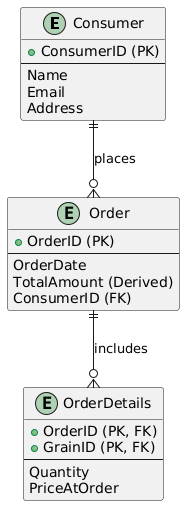
\includegraphics[height=0.5\textwidth]{CONSUMER_ER.png}
    \caption{Consumer Entity-Relationship Diagram (ERD)}
\end{figure}

\subsubsection{Suppliers Entity Sub-Diagram}

This diagram breaks down the \textbf{Order Entity}, representing how consumer orders are managed within the system.

\begin{figure}[htbp] % Relaxed float placement with 'htbp'
    \centering
    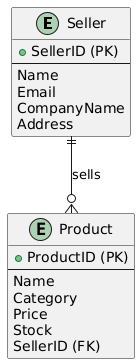
\includegraphics[height=0.5\textwidth]{sellerEr.png}
    \caption{supplier Entity-Relationship Diagram (ERD)}
\end{figure}
\newpage

\smallskip
\textbf{Explanation}:
\begin{itemize}
    \item The \textbf{Order Entity} has attributes like \texttt{orderID}, \texttt{consumerID}, \texttt{productID}, \texttt{quantity}, and \texttt{orderStatus}.
    \item \texttt{OrderStatus} includes states such as \textit{pending}, \textit{dispatched}, and \textit{delivered}.
    \item Each order is associated with a specific consumer, and the \texttt{consumerID} links the order back to the user's profile.
\end{itemize}
\section{Class Design}

\subsection{Overview}
The Class Design section defines the object-oriented structure of the Agri Vision system, detailing the classes, their attributes, methods, and the relationships between them. The primary goal is to ensure modularity and reusability while maintaining a clear separation of concerns between the different roles in the agricultural ecosystem (farmers, suppliers, consumers, etc.).

\subsection{Class Diagram}
The \textbf{Class Diagram} provides a high-level view of the main system classes, their relationships, and interactions within the Agri Vision platform.

\begin{figure}[htbp]
    \centering
    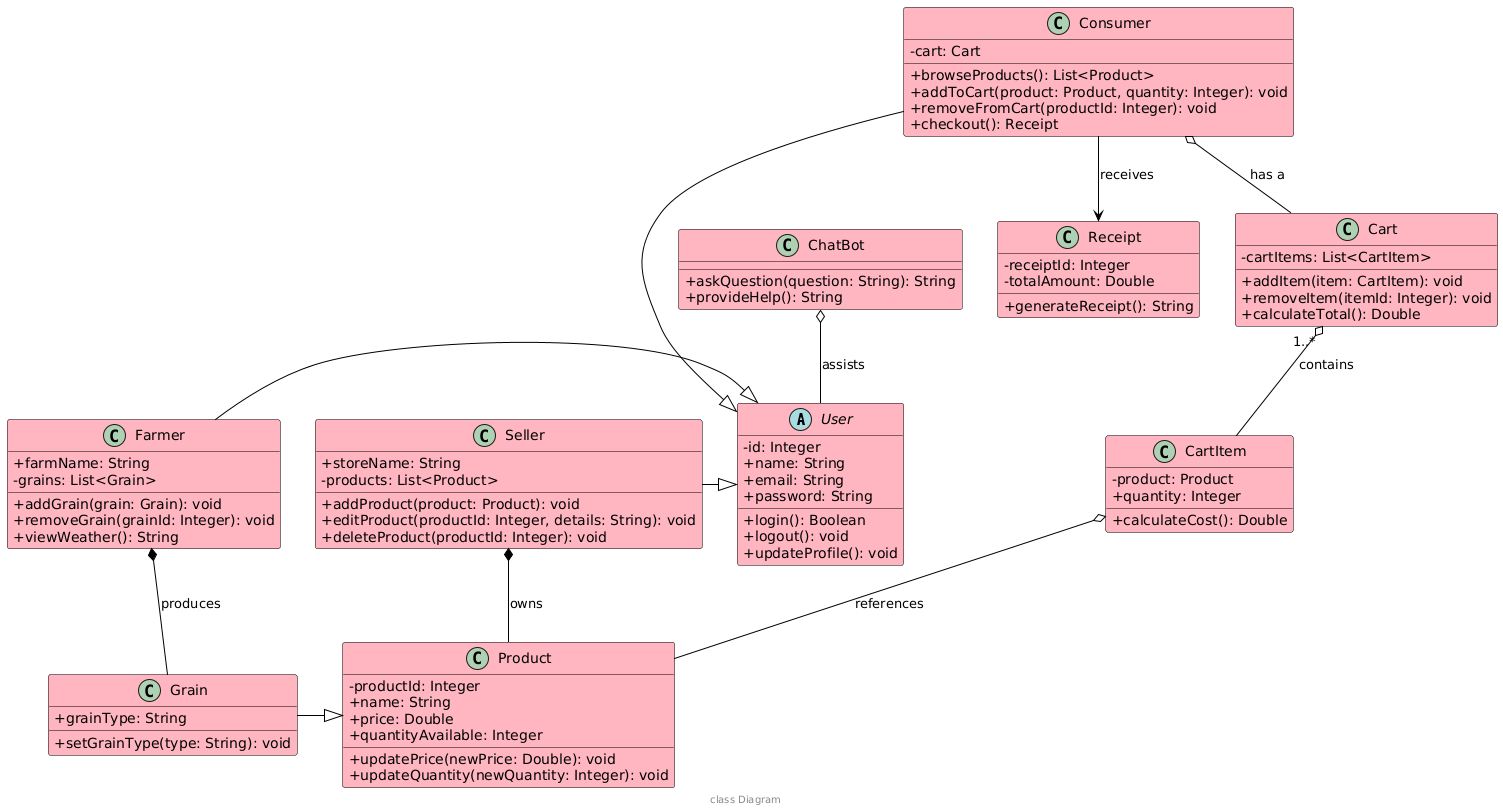
\includegraphics[width=1.1\textwidth]{classDiagram4.png}
    \caption{Main Class Diagram for Agri Vision}
    \label{fig:main_class_diagram_agri}
\end{figure}

\textbf{Explanation}:
\begin{itemize}
    \item The \textbf{User Class} manages the user-related data, including farmers, consumers, and suppliers.
    \item The \textbf{Product Class} represents the products (grains, seeds, pesticides, etc.) listed by suppliers and available for farmers and consumers.
    \item The \textbf{Transaction Class} tracks transactions between farmers, consumers, and suppliers (e.g., purchase, sale, rental).
    \item The \textbf{Weather Class} provides weather data associated with a user’s location (through the interactive map).
    \item Relationships between classes ensure proper data flow, such as the interaction between the \textbf{User Class} and the \textbf{Transaction Class} for managing purchases and sales.
\end{itemize}

\subsection{User Class Design}
% \begin{figure}[htbp]
%     \centering
%     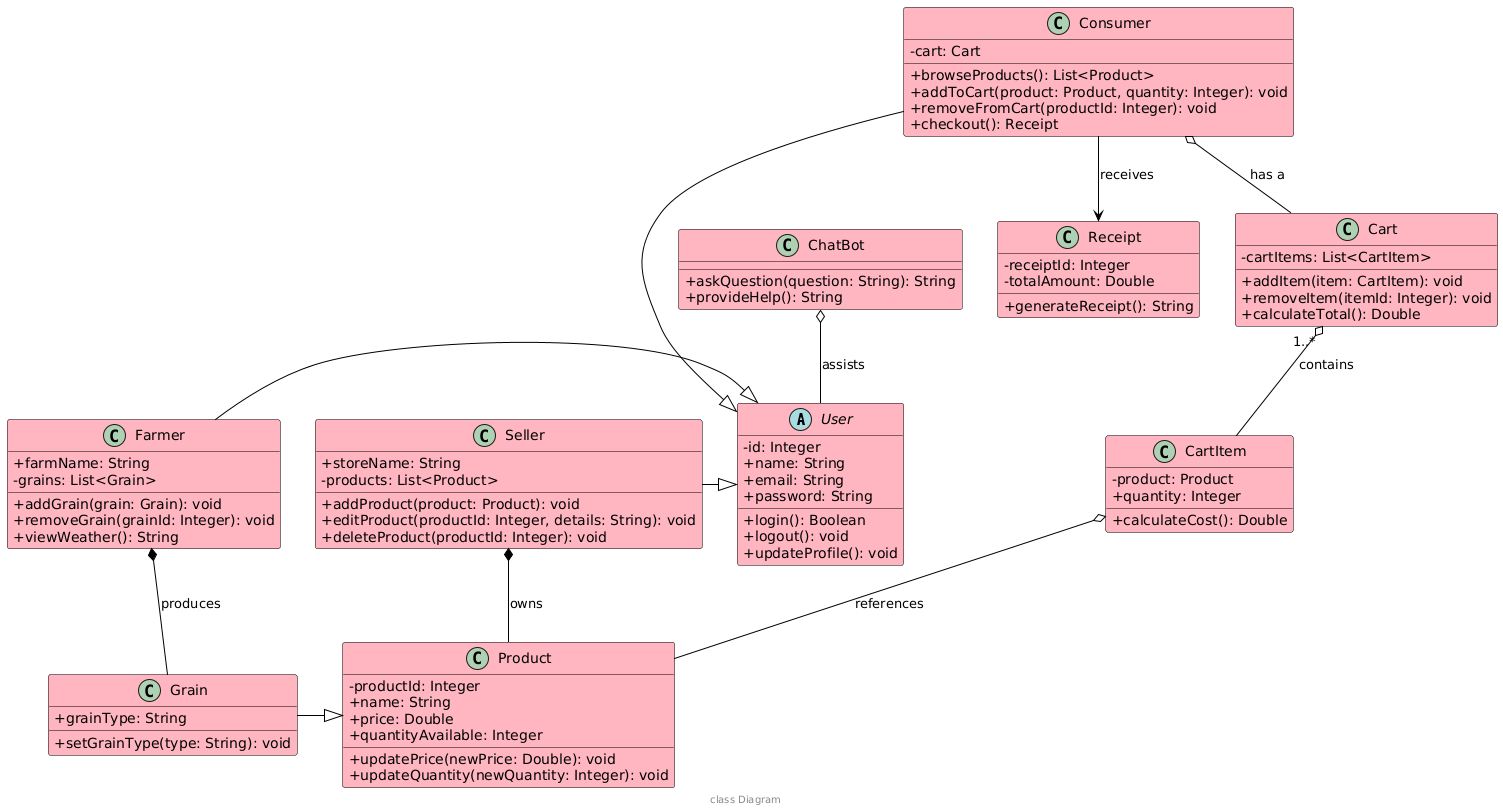
\includegraphics[height=0.1\textwidth]{classDiagram4.png}
%     \caption{User Class Design for Agri Vision}
%     \label{fig:user_class_agri}
% \end{figure}

\textbf{Explanation}:
\begin{itemize}
    \item \textbf{Attributes}:
        \begin{itemize}
            \item \texttt{userID}: A unique identifier for each user (farmer, supplier, consumer).
            \item \texttt{userType}: Specifies whether the user is a farmer, supplier, or consumer.
            \item \texttt{address}: The physical address of the user.
            \item \texttt{preferences}: Stores user-specific preferences, such as weather notifications and product recommendations.
        \end{itemize}
    \item \textbf{Methods}:
        \begin{itemize}
            \item \texttt{registerUser()}: Handles user registration for different user types.
            \item \texttt{updateProfile()}: Updates user details such as address or preferences.
            \item \texttt{viewProductList()}: Displays available products for purchase or rent (specific to user type).
        \end{itemize}
\end{itemize}

\subsection{Product Class Design}
% \begin{figure}[htbp]
%     \centering
%     \includegraphics[width=0.7\textwidth]{Product_Class_AgriVision.png}
%     \caption{Product Class Design for Agri Vision}
%     \label{fig:product_class_agri}
% \end{figure}

\textbf{Explanation}:
\begin{itemize}
    \item \textbf{Attributes}:
        \begin{itemize}
            \item \texttt{productID}: Unique identifier for each product.
            \item \texttt{productName}: The name of the product (e.g., wheat, pesticides).
            \item \texttt{price}: Price of the product.
            \item \texttt{category}: Specifies the type of product (e.g., grain, pesticide, machinery).
            \item \texttt{availability}: Indicates whether the product is available for sale or rent.
        \end{itemize}
    \item \textbf{Methods}:
        \begin{itemize}
            \item \texttt{addProduct()}: Allows suppliers to add new products to the marketplace.
            \item \texttt{updateProduct()}: Enables suppliers to edit product details (e.g., price, description).
            \item \texttt{removeProduct()}: Allows suppliers to remove products from the marketplace.
        \end{itemize}
\end{itemize}

% \subsection{Transaction Class Design}
% \begin{figure}[htbp]
%     \centering
%     \includegraphics[width=0.7\textwidth]{Transaction_Class_AgriVision.png}
%     \caption{Transaction Class Design for Agri Vision}
%     \label{fig:transaction_class_agri}
% \end{figure}

% \textbf{Explanation}:
% \begin{itemize}
%     \item \textbf{Attributes}:
%         \begin{itemize}
%             \item \texttt{transactionID}: A unique identifier for each transaction.
%             \item \texttt{productID}: The ID of the product involved in the transaction.
%             \item \texttt{buyerID}: The ID of the buyer (farmer or consumer).
%             \item \texttt{sellerID}: The ID of the seller (supplier).
%             \item \texttt{transactionType}: Specifies whether the transaction is a sale, rental, or purchase.
%             \item \texttt{transactionDate}: Timestamp of the transaction.
%         \end{itemize}
%     \item \textbf{Methods}:
%         \begin{itemize}
%             \item \texttt{createTransaction()}: Creates a new transaction record for a purchase or rental.
%             \item \texttt{viewTransactionHistory()}: Retrieves the transaction history for a user (buyer or seller).
%             \item \texttt{cancelTransaction()}: Allows users to cancel a transaction before completion.
%         \end{itemize}
% \end{itemize}

\subsection{Weather Class Design}
% \begin{figure}[htbp]
%     \centering
%     \includegraphics[width=0.7\textwidth]{Weather_Class_AgriVision.png}
%     \caption{Weather Class Design for Agri Vision}
%     \label{fig:weather_class_agri}
% \end{figure}

\textbf{Explanation}:
\begin{itemize}
    \item \textbf{Attributes}:
        \begin{itemize}
            \item \texttt{location}: The geographical location (latitude, longitude) of the user.
            \item \texttt{temperature}: The current temperature at the user's location.
            \item \texttt{humidity}: The current humidity level at the user's location.
            \item \texttt{forecast}: Weather forecast data for the next 24 hours.
        \end{itemize}
    \item \textbf{Methods}:
        \begin{itemize}
            \item \texttt{getWeatherData()}: Retrieves the current weather data based on the user's location.
            \item \texttt{getWeatherForecast()}: Retrieves the 24-hour weather forecast for the user's location.
        \end{itemize}
\end{itemize}


\newpage












\section{Interaction Design}

\subsection{Sequence Diagram}
The \textbf{Sequence Diagram} provides a detailed view of how system components interact during specific operations. It visualizes the order of interactions and highlights the system's dynamic behavior.

\begin{figure}[htbp]
    \centering
    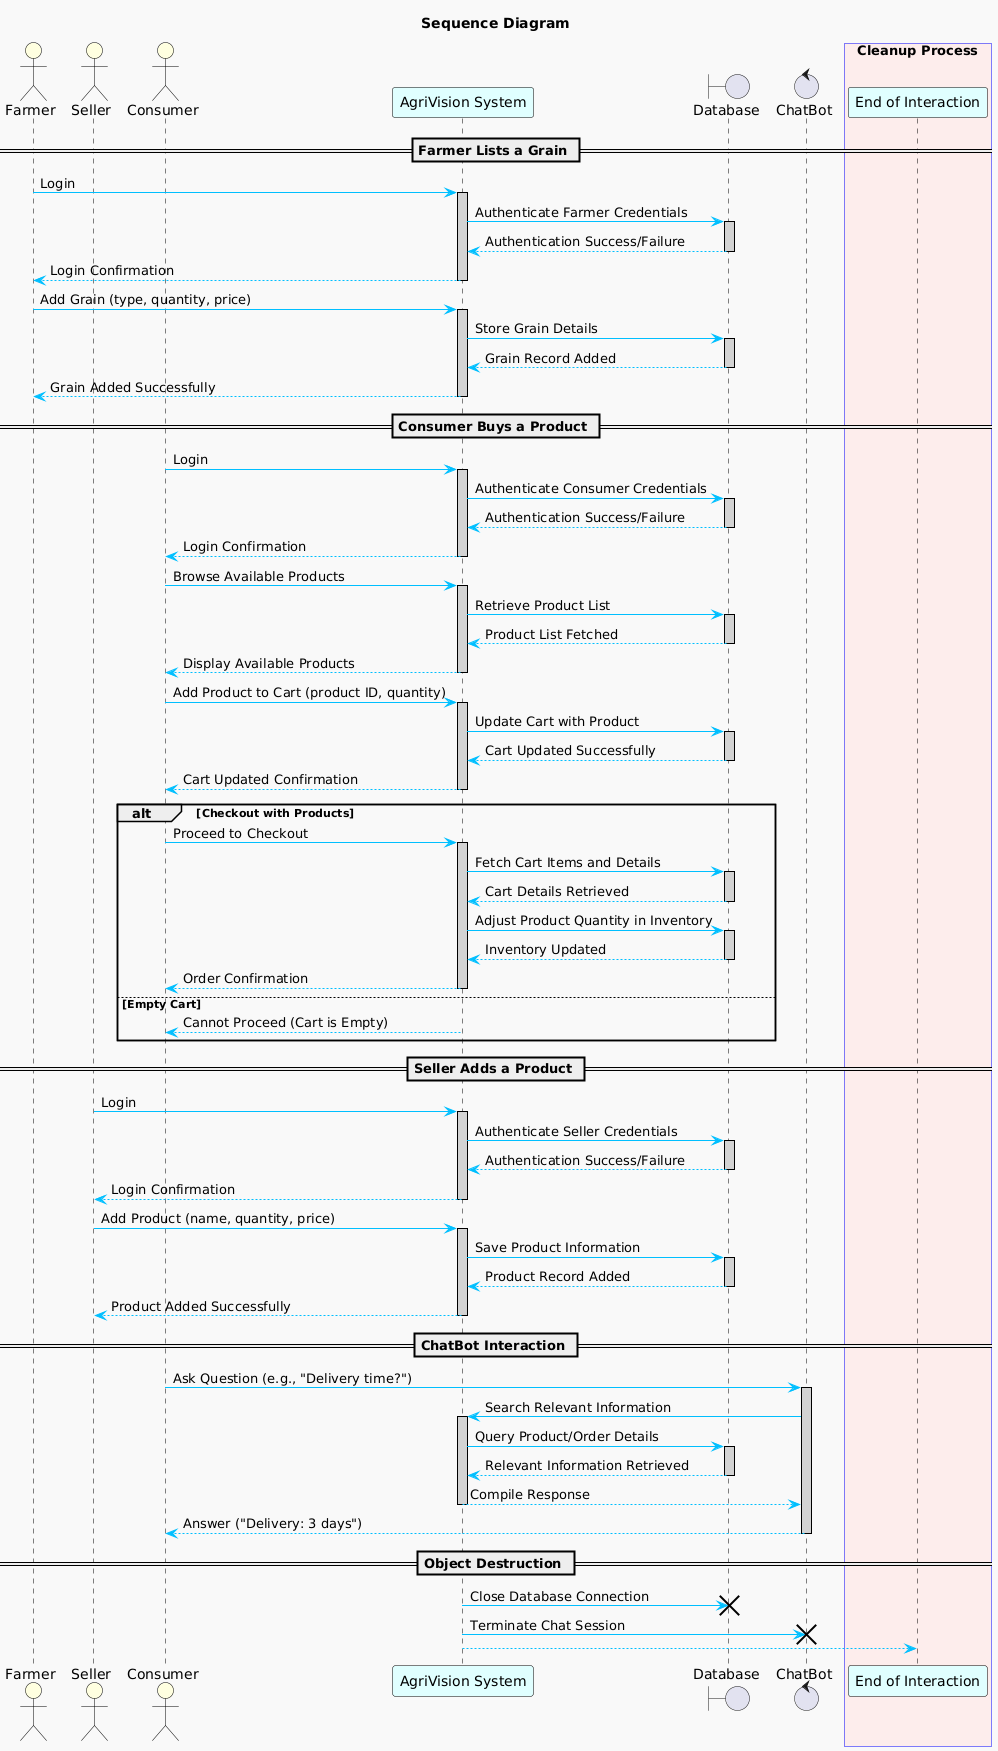
\includegraphics[width=0.8\textwidth]{newseq.png}
    \caption{Sequence Diagram}
    \label{fig:user_registration_sequence}
\end{figure}

\textbf{Explanation}:
\begin{itemize}
    \item The sequence diagram illustrates the process of user registration in the system:
        \begin{itemize}
            \item The user initiates the process by submitting their registration details through the front-end interface.
            \item The server validates the user's input, ensuring all required fields are correctly filled and follow predefined rules.
            \item Once validated, the server communicates with the database to store the user’s information.
            \item The user receives feedback confirming successful registration.
        \end{itemize}
\end{itemize}

\newpage

\subsection{Sub-Diagrams}

\subsubsection{Farmer Sequence Diagram}
This sub-diagram demonstrates the steps the system follows to detect vulnerabilities.

\begin{figure}[htbp]
    \centering
    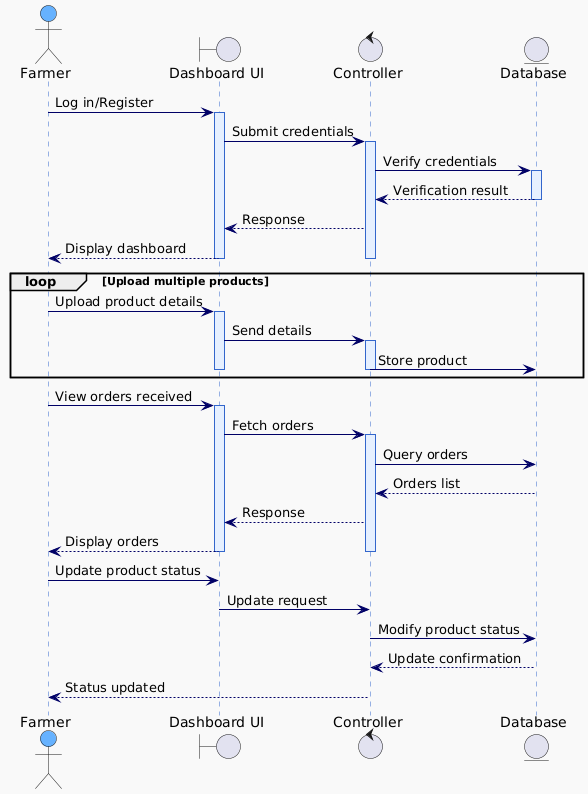
\includegraphics[width=0.8\textwidth]{farmerseq.png}
    \caption{Sequence for Farmer}
    \label{sequence_farmer}
\end{figure}

\textbf{Explanation}:
\begin{itemize}
    \item The sequence begins with the system initiating a scan on websites for vulnerabilities related to agricultural products and services.
    \item Detected vulnerabilities are sent to the backend for detailed analysis and categorization.
    \item The backend evaluates the severity of each vulnerability, prioritizing issues that may affect farmer activities.
    \item Results are stored in the database for further reference and reporting.
    \item The system triggers notifications to relevant users, including farmers, about critical vulnerabilities in their profiles.
\end{itemize}


\subsubsection{Consumer Sequence Diagram}
This diagram details how the system handles notifications when a vulnerability is detected.

\begin{figure}[htbp]
    \centering
    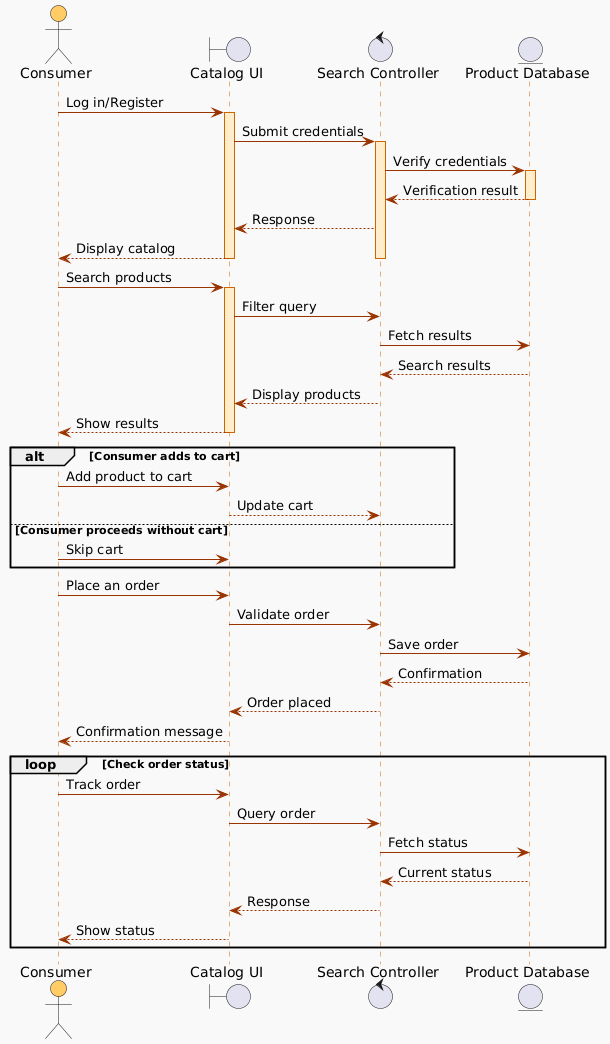
\includegraphics[width=0.8\textwidth]{consumerseq.png}
    \caption{Sequence for Consumers}
    \label{fig:vulnerability_detection_sequence_consumer}
\end{figure}

\textbf{Explanation}:
\begin{itemize}
    \item The system identifies consumers affected by a detected vulnerability.
    \item The backend prepares the notification message with relevant details about the vulnerability.
    \item The system sends the notification to consumers via their registered communication channels (e.g., email, SMS).
    \item Consumers receive the notification and can view more details about the vulnerability by accessing the application.
\end{itemize}

\newpage

\subsubsection{Supplier Sequence Diagram}
This diagram demonstrates the steps involved when a vulnerability is detected for a supplier’s profile or product.

\begin{figure}[htbp]
    \centering
    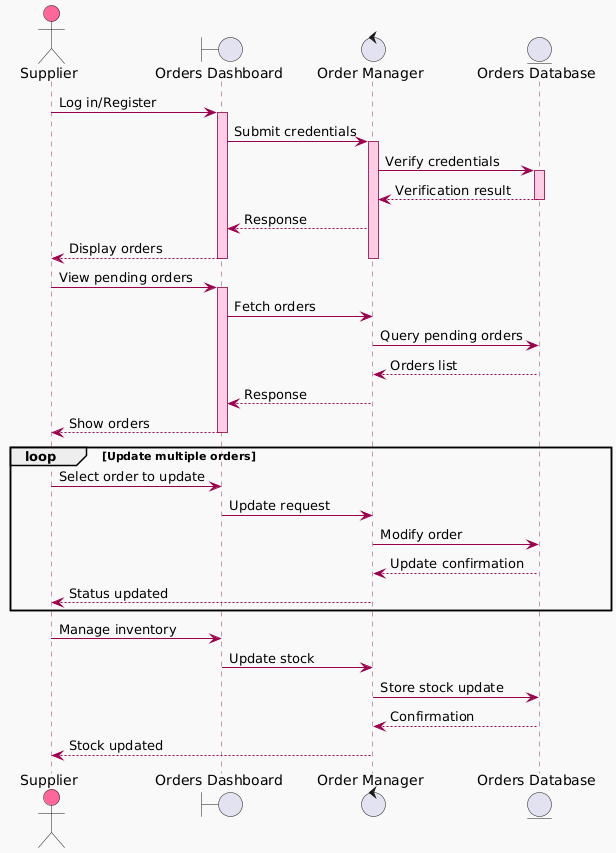
\includegraphics[width=0.9\textwidth]{supplierseq.png}
    \caption{Sequence for Suppliers}
    \label{fig:vulnerability_detection_sequence_supplier}
\end{figure}

\textbf{Explanation}:
\begin{itemize}
    \item The system identifies suppliers whose products or profiles are affected by a detected vulnerability.
    \item The backend prepares the notification message, which includes the vulnerability details, and identifies if there is a need to update product listings or secure profiles.
    \item Notifications are sent to the suppliers via registered communication channels (e.g., email, SMS).
    \item Suppliers receive the notification and can take necessary actions, such as updating their product listings or profiles, to mitigate vulnerabilities.
\end{itemize}
\newpage



\section{Data Flow Design}

\subsection{Data Flow Diagram}

The \textbf{Data Flow Diagram (DFD)} provides a high-level overview of how data flows within the system. It shows the input, processes, storage, and output of the data.

\subsubsection{Level 0}

The Level 0 DFD illustrates the system's overall data flow, focusing on the interactions between external entities and the main processes in the Agri Vision project.

\begin{figure}[h]
    \centering
    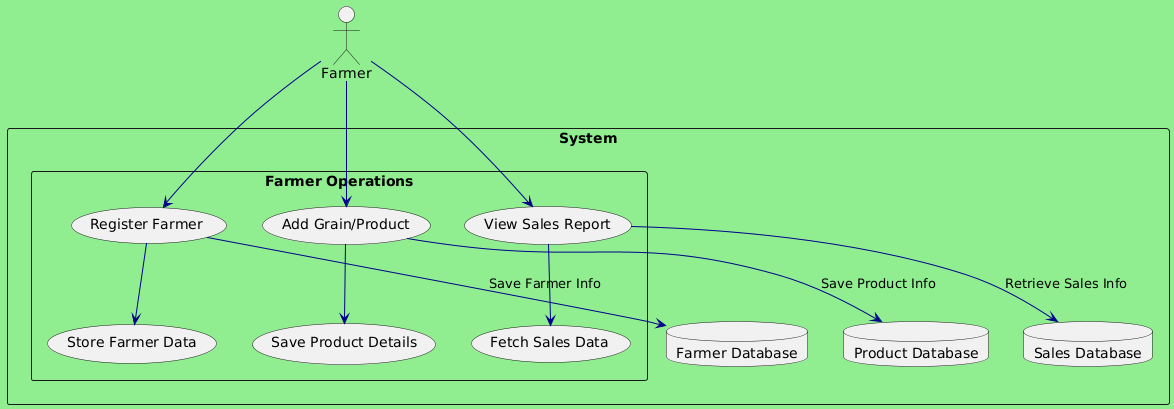
\includegraphics[width=1.1\textwidth]{farmerflow.png}
    \caption{Data flow at farmer}
\end{figure}

\textbf{Explanation}:
\begin{itemize}
    \item \textbf{Entities}:
        \begin{itemize}
            \item \textbf{User}: Interacts with the system, performing actions like registering, managing profiles, and accessing weather updates.
          
        \end{itemize}
    \item \textbf{Processes}:
        \begin{itemize}
            \item \textbf{Agri Vision System (AVS)}: Handles data processing, including user registrations, product management, weather reporting, and profile management.
        \end{itemize}
    \item \textbf{Data Flow}:
        \begin{itemize}
            \item Users submit requests such as product updates, profile changes, or location-based weather queries.
            \item The system processes the data, stores it in the database, and triggers relevant notifications to the user (e.g., updates on products or weather conditions).
        \end{itemize}
\end{itemize}

\newpage

\subsubsection{Level 1}

This sub-diagram details the primary processes within the Agri Vision system, such as user registration, weather data collection, vulnerability detection, and profile management.

\begin{figure}[h]
    \centering
    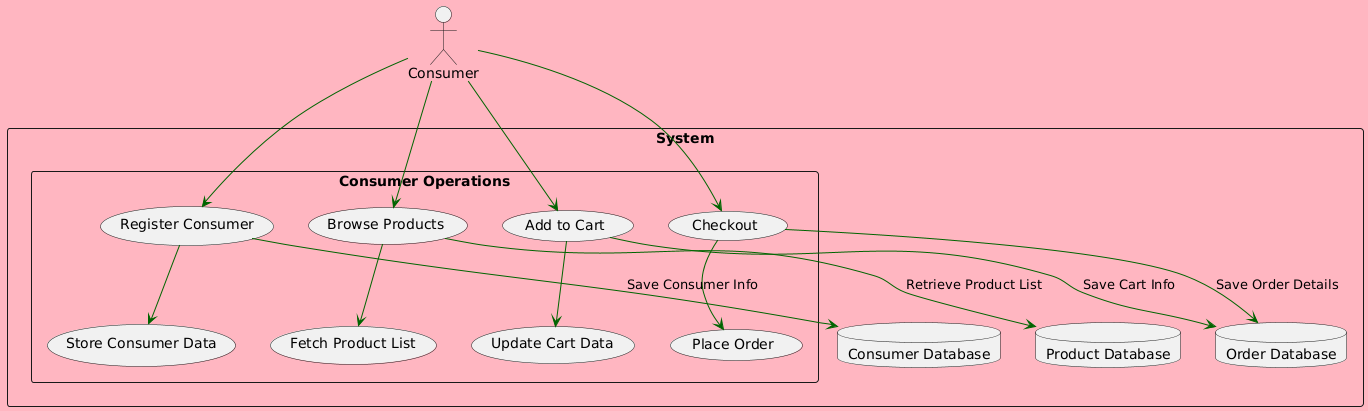
\includegraphics[width=1.1\textwidth]{consumerflow.png}
    \caption{Data flow at Consumer}
\end{figure}

\textbf{Explanation}:
\begin{itemize}
    \item \textbf{Processes}:
        \begin{itemize}
            \item \textbf{User Registration}: Captures the user's details and stores them in the system.
            \item \textbf{Weather Data Collection}: Gathers weather information based on user location or map interactions.
            \item \textbf{Vulnerability Detection}: Scans agricultural products for vulnerabilities, like pests or diseases, and updates the database.
            \item \textbf{Profile Management}: Allows users (farmers, sellers, consumers) to add, edit, or delete profiles and products.
        \end{itemize}
    \item \textbf{Data Flow}:
        \begin{itemize}
            \item Users submit their registration, product details, or weather queries to the system.
            \item The system processes this data, stores it in the database, and triggers notifications (e.g., weather alerts or product updates).
        \end{itemize}
\end{itemize}


\subsection{Sub-Diagrams}
\begin{figure}[h]
    \centering
    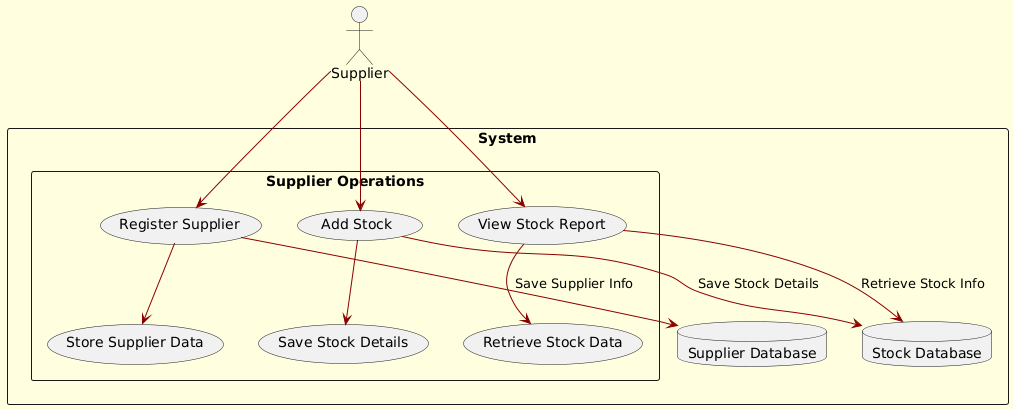
\includegraphics[width=1.1\textwidth]{supplierdflow.png}
    \caption{Data flow at supplier.}
\end{figure}

\textbf{Explanation}:
\begin{itemize}
    \item \textbf{Scan Agricultural Products}: Initiates a scan to check for vulnerabilities (e.g., pests, diseases) affecting crops or seeds.
    \item \textbf{Analyze Results}: Processes scanned data to identify risks like pests, soil quality, or environmental issues.
    \item \textbf{Store Vulnerability Data}: Saves vulnerability findings to the database for further reporting.
    \item \textbf{Data Flow}:
        \begin{itemize}
            \item The system scans and processes data related to agricultural products.
            \item The findings are stored and retrieved as needed, generating alerts or updates.
        \end{itemize}
\end{itemize}


\subsubsection{Weather Data Collection Sub-DFD}

This sub-diagram focuses on how weather data is collected, processed, and displayed to the user based on location.

% \begin{figure}[h]
%     \centering
%     \includegraphics[width=1.1\textwidth]{weatherflow.png}
%     \caption{Weather Data Collection Data Flow Diagram}
% \end{figure}

\textbf{Explanation}:
\begin{itemize}
    \item \textbf{Request Weather Information}: The user submits a location to retrieve the weather data.
    \item \textbf{Fetch Weather Data}: The system connects to weather APIs to collect data.
    \item \textbf{Display Weather Data}: The system processes and presents weather data to the user in the interface.
    \item \textbf{Data Flow}:
        \begin{itemize}
            \item The user's location is used to fetch relevant weather data.
            \item Weather data is processed and displayed on the map or user interface.
        \end{itemize}
\end{itemize}


% 7th section

\section{Activity Design}

\subsection{Activity Diagram}
The \textbf{Activity Diagram} represents the dynamic aspects of the system, illustrating the flow of activities within various processes in the Agri Vision project.

\begin{figure}[htbp]
    \centering
    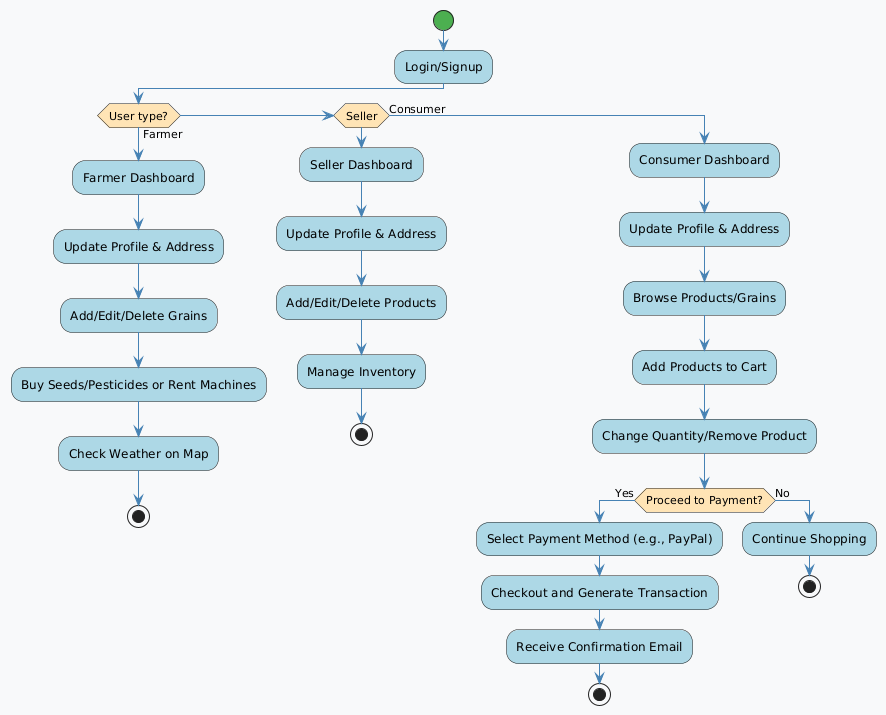
\includegraphics[width=1.1\textwidth]{activity.png}
    \caption{Main Activity Diagram: User Interaction Flow}
\end{figure}
\textbf{Explanation:}
\begin{itemize}
    \item \textbf{User Interaction:} 
    The user initiates the workflow by submitting requests for weather data, product updates, or profile management.
    \item \textbf{Weather Data Retrieval:} 
    Based on the user's location or interaction with the map, the system retrieves weather data from external APIs.
    \item \textbf{Profile Management:} 
    Users interact with their profile (e.g., update address, manage products) and make changes.
    \item \textbf{Vulnerability Detection (if applicable):} 
    The system may also initiate vulnerability scans for products (e.g., crops or seeds) and store the results in the database.
    \item \textbf{Notification Trigger:} 
    Based on the weather data, product updates, or vulnerabilities, notifications are prepared and sent to users.
    \item \textbf{Database Update:} 
    All processed information, such as weather data, product details, or vulnerabilities, is stored in the database for future reference.
\end{itemize}

\subsection{Sub-Diagrams}

\subsubsection{Activity Diagram: Admin Process}
This diagram elaborates on the internal steps for managing user accounts, updating product information, and overseeing the system's operations.

\begin{figure}[h]
    \centering
    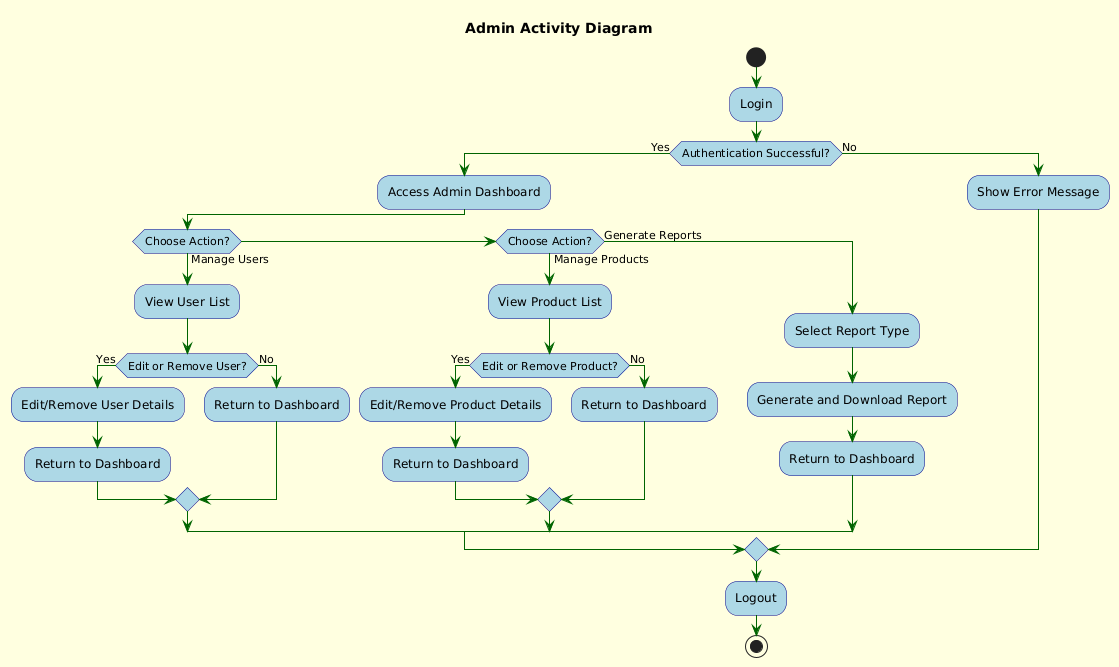
\includegraphics[width=1.2\textwidth]{adminActivity.png}
    \caption{Admin Process Activity Diagram}
\end{figure}
\textbf{Explanation:}
\begin{itemize}
    \item The admin system begins by receiving requests for user registration or product updates.
    \item It checks for the validity of the requests, such as ensuring that users are registered or verifying that product details are accurate.
    \item The system may trigger vulnerability scans for certain products or monitor the system for performance and security issues.
    \item The admin can update the database with new product listings, user details, or critical system notifications.
\end{itemize}





\subsubsection{Activity Diagram: User Registration Process}
This diagram illustrates the activity flow for user registration, which is essential for farmers, sellers, and consumers.

% \begin{figure}[htbp]
%     \centering
%     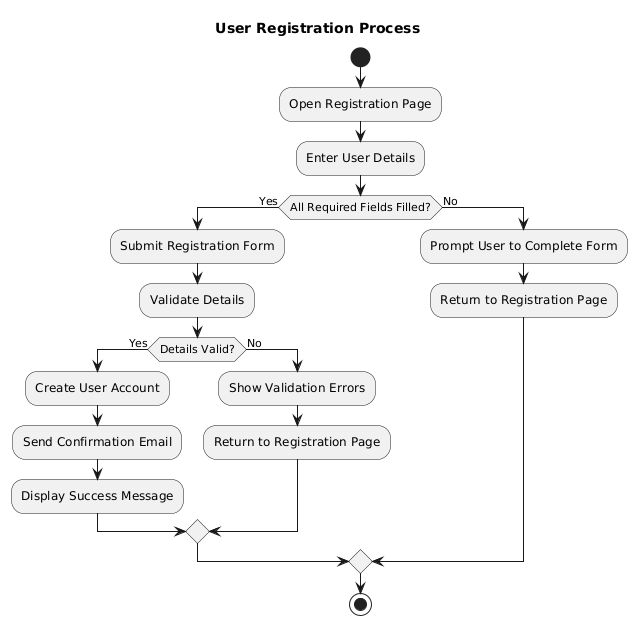
\includegraphics[width=0.1\textwidth]{userRegister.png}
%     \caption{User Registration Activity Diagram}
% \end{figure}

\textbf{Explanation:}
\begin{itemize}
    \item The user provides registration details, including personal information and preferences.
    \item The system validates the input data for correctness and ensures that the data is not already in the system.
    \item Upon successful validation, the user's details are stored in the database.

\end{itemize}




\newpage















\section{Frontend Images}
\begin{itemize}
    \item The subject line is concise and highlights the purpose of the email, such as \textbf{Order Confirmation}, \textbf{Profile Update}, or \textbf{New Product Listing Notification}.
    \item Key details (e.g., order ID, update summary, or relevant dates) ensure users have all necessary information at a glance.
    \item The email includes direct links to the Agri Vision dashboard, allowing users to view their orders, update their profiles, or access additional resources.
\end{itemize}

\subsection{Frontend Images}
Below are sample screenshots of the Agri Vision user interface:

\begin{itemize}
    \item \textbf{Farmer Dashboard:} A streamlined view for farmers to list grains, edit personal/company details, and access farming resources like weather updates or machinery rentals.
    \item \textbf{Seller Interface:} A dedicated space for sellers to manage product inventories, update addresses, and interact with consumers.
    \item \textbf{Consumer Interface:} A user-friendly section for consumers to browse agricultural products, manage carts, and finalize purchases with farmers or sellers.
\end{itemize}

These images illustrate the intuitive and role-specific designs that make the platform efficient and user-friendly for all stakeholders.


\begin{figure}[htbp]
    \centering
    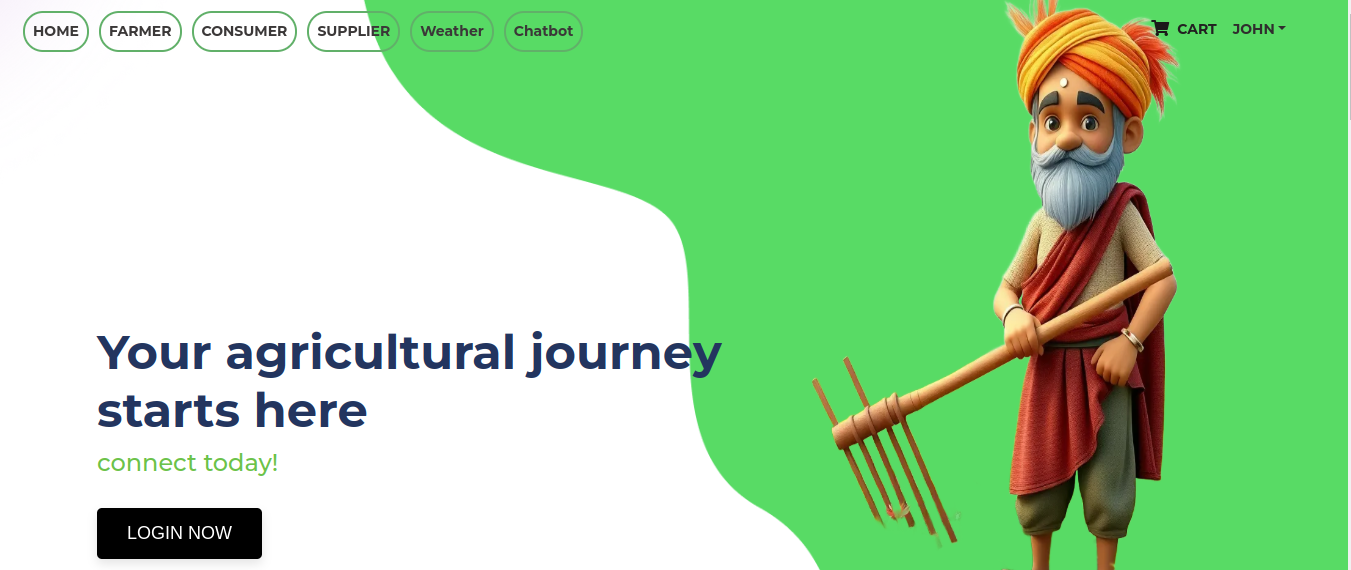
\includegraphics[width=1.1\textwidth]{herosecnew.png}
    \caption{Agri vision Landing Page}
    \label{fig:dashboard}
\end{figure}
\begin{figure}[htbp]
    \centering
    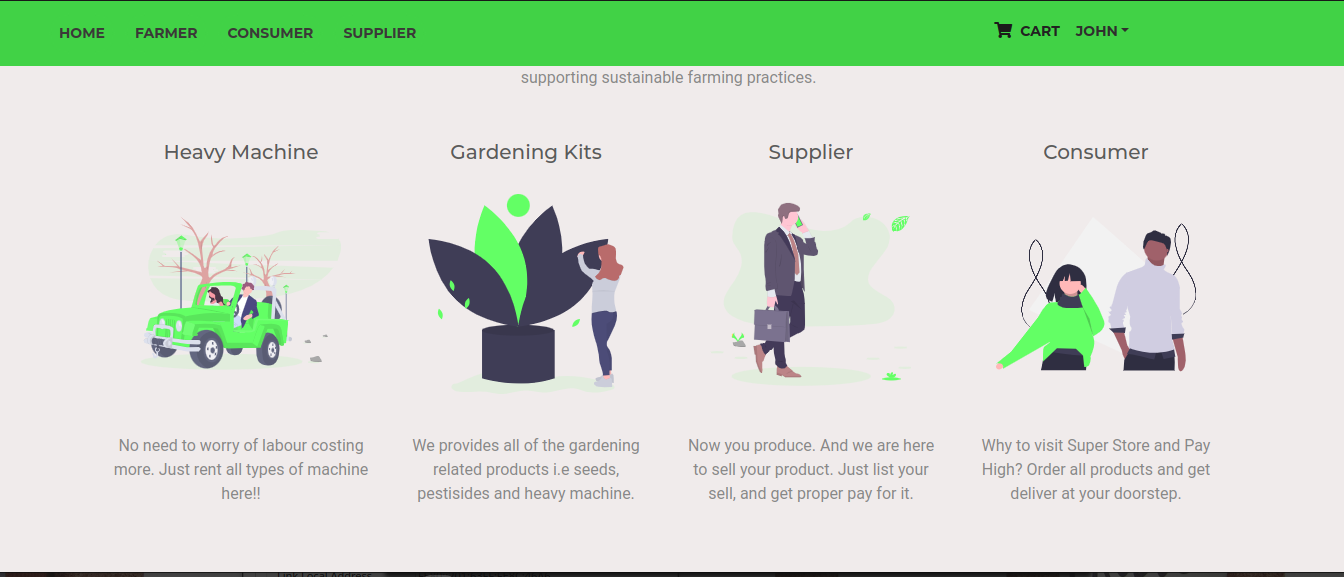
\includegraphics[width=1.1\textwidth]{agri/interfaces2.png}
    \caption{Landing page of AgriVision}
    \label{fig:dashboard}
\end{figure}


\begin{figure}[htbp]
    \centering
    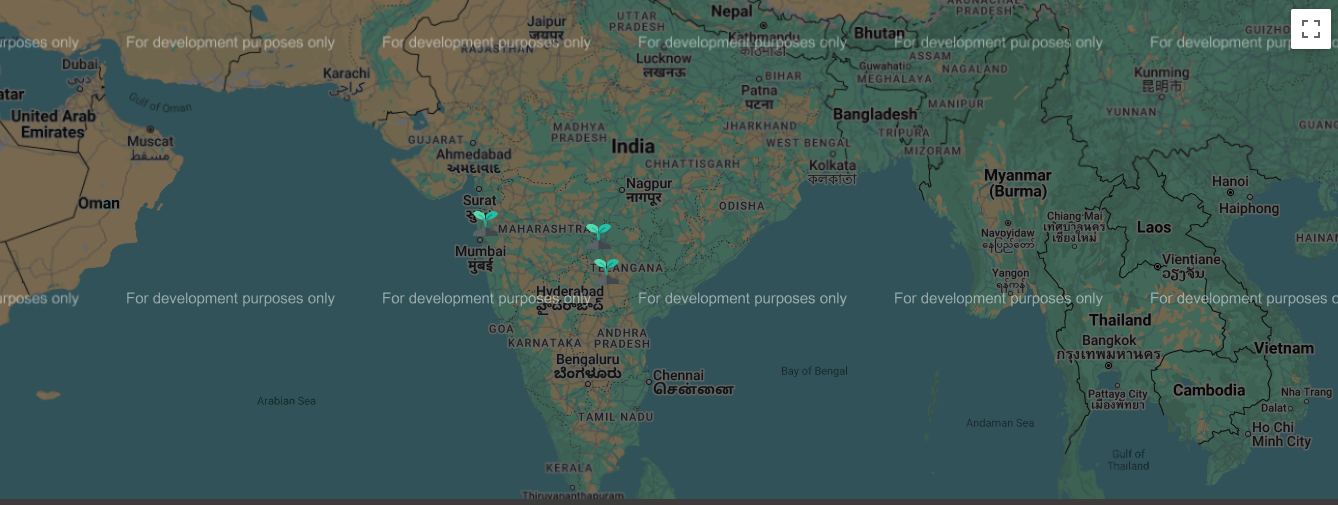
\includegraphics[width=1.1\textwidth]{agri/map.png}
    \caption{weather map}
    \label{fig:dashboard}
\end{figure}


\begin{figure}[htbp]
    \centering
    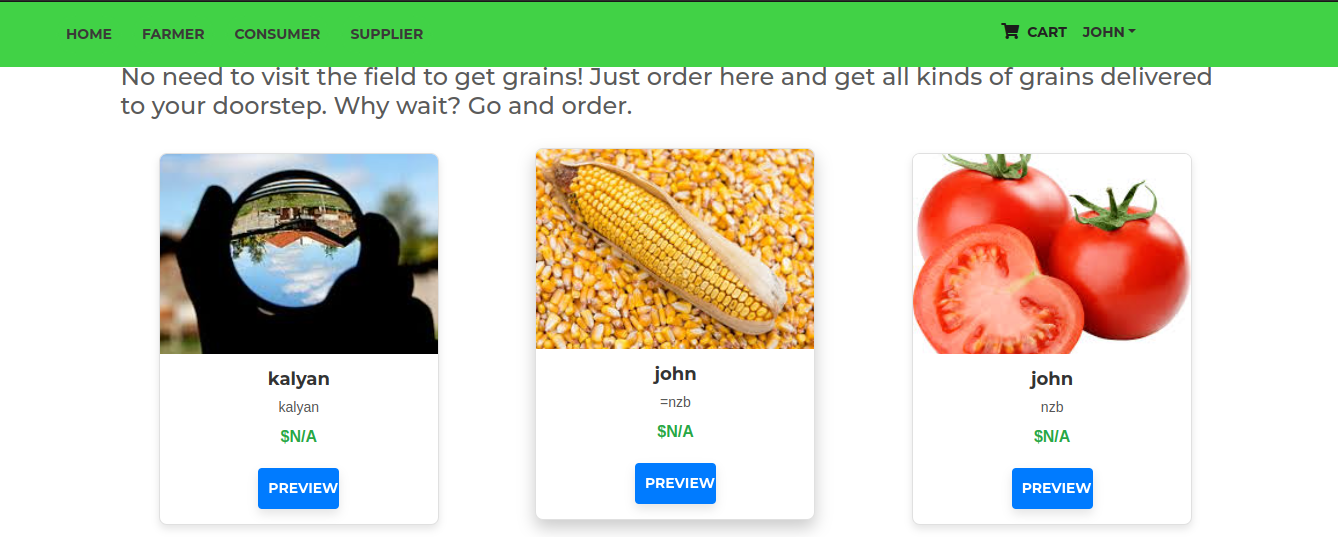
\includegraphics[width=1.1\textwidth]{agri/consumers3.png}
    \caption{Consumer section}
    \label{fig:dashboard}
\end{figure}

\begin{figure}[htbp]
    \centering
    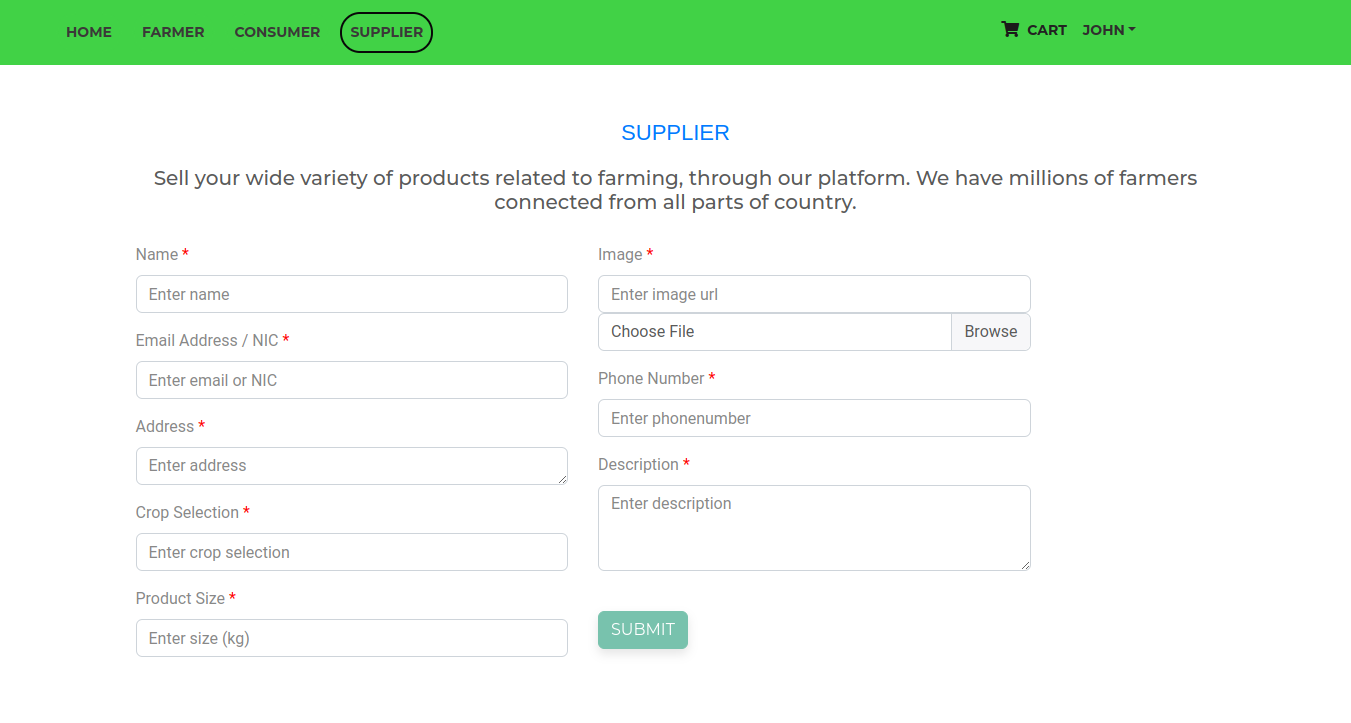
\includegraphics[width=1.1\textwidth]{suppliers3.png}
    \caption{Supplier section}
    \label{fig:dashboard}
\end{figure}


\begin{figure}[htbp]
    \centering
    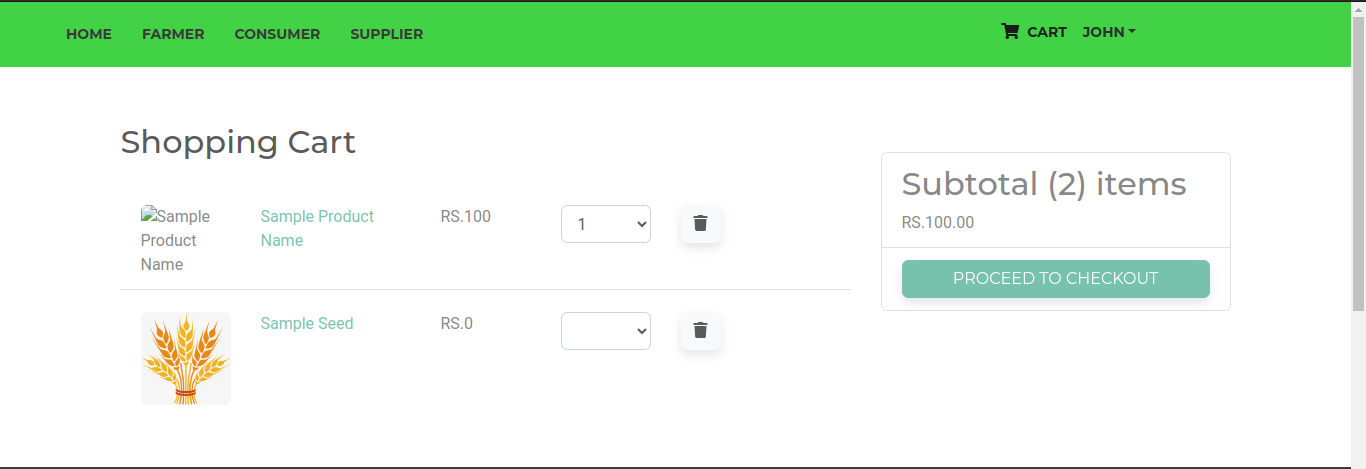
\includegraphics[width=1.1\textwidth]{agri/carts1.png}
    \caption{Cart section}
    \label{fig:dashboard}
\end{figure}



\begin{figure}[htbp]
    \centering
    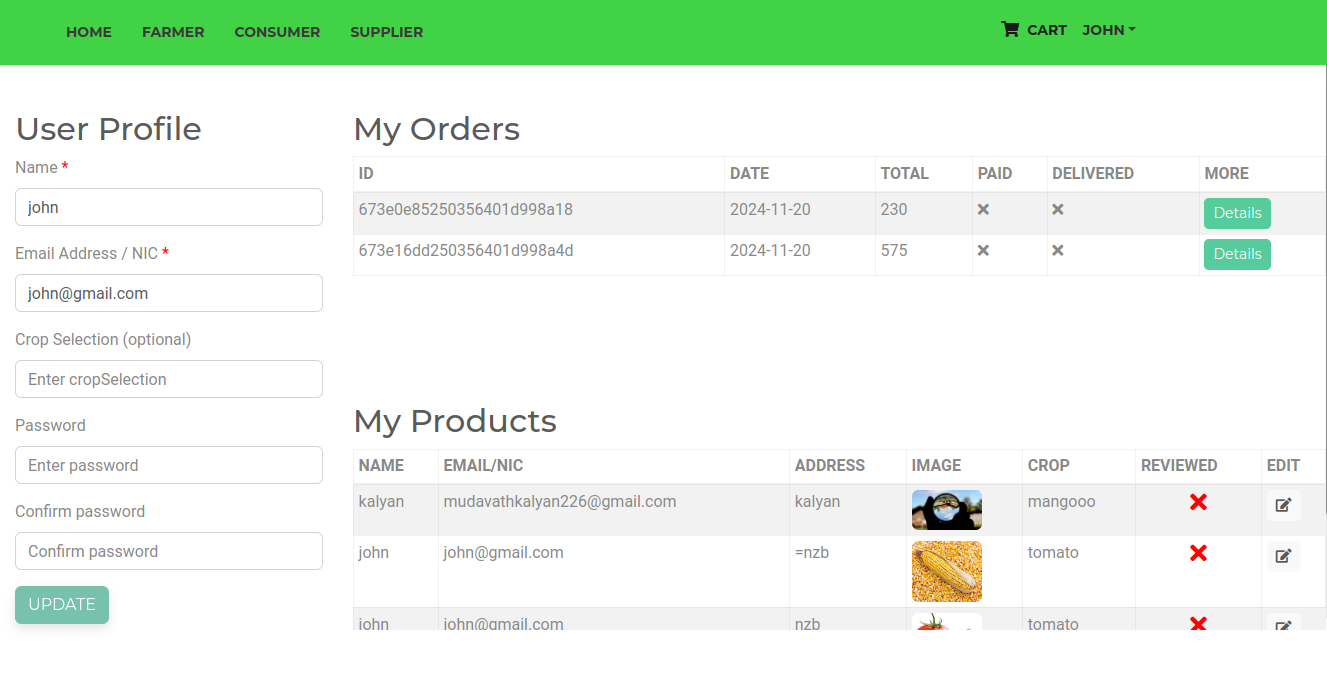
\includegraphics[width=1.1\textwidth]{profilesec2.png}
    \caption{Profile section}
    \label{fig:dashboard}
\end{figure}








\newpage
\subsection{Conclusion}
The Agri Vision Platform revolutionizes the agricultural ecosystem by creating a unified space for farmers, sellers, and consumers to connect seamlessly. By eliminating intermediaries, it ensures fair pricing for farmers while offering consumers access to fresh, organic products directly from the source. Farmers can also access essential tools like weather updates and resources such as seeds, pesticides, and machinery rentals, empowering them for better productivity.

Sellers gain an efficient platform to manage inventory and expand their reach, while consumers enjoy simplified interactions with transparent access to agricultural goods. Agri Vision addresses key challenges like market fragmentation and inefficiencies, fostering a fair, sustainable, and digitally driven agricultural ecosystem that empowers communities and promotes equitable growth.


\end{document}
